% -*- mode: latex; fill-column: 80; -*-
\documentclass[a4paper,10pt]{report}

\usepackage{hyperref}
\hypersetup{
  colorlinks,
  citecolor=blue,
  filecolor=blue,
  linkcolor=blue,
  urlcolor=blue
}

\usepackage{graphicx}
\graphicspath{ {./image/} }

\usepackage{subcaption}

\def\FlintVersion{1.8}
\def\Flint{Flint \FlintVersion}

\newcommand\FigureOfImage[2]{\begin{figure}[h]
  \centering
  \includegraphics[width=0.6\textwidth]{#1}
  \caption{#2}\label{fig:#1}
\end{figure}}

\title{\Flint: The User Guide}
\author{Flint project}

\makeindex

\begin{document}

\maketitle

\begin{abstract}
This document describes how to use \Flint.
Readers also find some OS-specific notes and trouble-shooting techniques which
users would like to know when using \Flint.
\end{abstract}

\tableofcontents


%%%%%%%%%%%%%%%%%%%%%%%%%%%%%%%%%%%%%%%%%%%%%%%%%%%%%%%%%%%%%%%%%%%%%%%%

\chapter{Introduction}
Welcome to \Flint.

\section{Brief summary about Flint}
Flint can run simulations of multi-level physiological models written in PHML.
It means that Flint parses given models, performs numerical analysis for their
simulation, and renders simulation outcome into a line graph on the plot
window's canvas. Likewise, Flint can handle SBML and SBML-PHML hybrid models.
Furthermore, Flint offers a plug-in feature with which different types of
plotting applications such as gnuplot are available.

\subsection{Markup languages}
\Flint\ supports the following three languages for models:
\begin{itemize}
\item PHML/ISML
\item SBML
\end{itemize}

\subsection{Solver methods for ordinary differential equations}
\Flint\ supports the following two algorithms to solve ODEs numerically:
\begin{itemize}
\item Euler method
\item Runge-Kutta 4th-order method
\item Adaptive stepsize Runge-Kutta method, based on the ARKode solver of SUNDIALS
\end{itemize}

\section{Notation}
In this document, a sentence starting with {\tt \$} describes a command line in
a command shell on your system, such as\\
{\tt \$ echo this is a command line.}


%%%%%%%%%%%%%%%%%%%%%%%%%%%%%%%%%%%%%%%%%%%%%%%%%%%%%%%%%%%%%%%%%%%%%%%%

\chapter{Getting started}

\section{Install \Flint}
Flint project makes both Windows and macOS version of \Flint\ freely
available at \url{https://flintproject.github.io/}.
The .dmg archive for macOS contains Flint's application bundle, named
``Flint.app''; extracting it and copying it into your favorite path is all
you have to do for installation.
For Windows, double-clicking the .msi package will start the installation
process.

\section{Try your first simulation with \Flint}
This section describes a simple procedure with \Flint\ to run a simulation of a
sample model ``HodgkinHuxley\_1952\_neuron\_model.phml'', which is distributed
as part of the PhysioDesigner installation.

\begin{description}
\item[Launch Flint] \hfill \\
To launch Flint, double-click flint.exe on Windows, or Flint.app on macOS.
\FigureOfImage{initial}{The initial window of Flint.}

\item[Open a model] \hfill \\
In the ``File'' menu, select ``Open'' to choose a model file. Then you will see
a file dialog like Fig.~\ref{fig:open-model}.
\FigureOfImage{open-model}{The file dialog to open a model.}
Select ``HodgkinHuxley\_1952\_neuron\_model.phml'' in the file dialog, and
click ``Open'' button. Then the model window will appear like Fig.~\ref{fig:hh}.
\FigureOfImage{hh}{The model window.}

\item[Choose duration and time step] \hfill \\
Specify the duration of simulation in ``Simulation Length'' and the time step
length of the simulation in ``Simulation Time Step'' optionally.

\item[Run a simulation] \hfill \\
Click the ``Run'' button to start a simulation.

Once simulation started running, the progress bar will appear in the control
panel in the right side like Fig.~\ref{fig:hh-progress}, and both ``Cancel''
(with the cross mark) and ``Detail'' buttons will be enabled.
\FigureOfImage{hh-progress}{The progress bar for the model.}

Wait until a message dialog shows up to tell that the simulation completed.
\FigureOfImage{hh-completed}{The message dialog says the simulation completed.}

\item[See detail of the simulation] \hfill \\
Click the ``Detail'' button to get the simultion result.
Then a detail window will appear like Fig.~\ref{fig:hh-detail}.
\FigureOfImage{hh-detail}{The detail window.}

\item[Select ordinates] \hfill \\
Click the ``View'' button on the detail window, then a plot window to render
line graphs about the simulation result, like Fig.~\ref{fig:hh-plot}.
\FigureOfImage{hh-plot}{The plot window.}
Drag a name card ``V'' from the variable list, and drop it into the right axis
field labelled Y1. Soon the corresponding line graph will appear on the canvas,
like Fig.~\ref{fig:hh-plot-v}.
\FigureOfImage{hh-plot-v}{The plot window with ``V'' on Y1.}
At the same time you can also pick up another name ``I\_Na'' from the list,
moving it into the left axis field labelled Y2, like
Fig.~\ref{fig:hh-plot-v-ina}.
\FigureOfImage{hh-plot-v-ina}{The plot window with ``V'' on Y1 and ``I\_Na''
on Y2.}

\item[Plot a line graph with gnuplot] \hfill \\
Push button ``Plot'' to draw the line graph about ``V'' and ``I\_Na'' with
gnuplot. Soon a gnuplot window will pop up like Fig.~\ref{fig:hh-gnuplot}.
\FigureOfImage{hh-gnuplot}{Line graph by gnuplot about ``V'' and ``I\_Na''.}
\end{description}


%%%%%%%%%%%%%%%%%%%%%%%%%%%%%%%%%%%%%%%%%%%%%%%%%%%%%%%%%%%%%%%%%%%%%%%%

\chapter{Graphical User Interface}
\Flint\ comes with a graphical user interface out of the box. This chapter
explains features of the GUI and how to use them.

\section{Launching Flint}
On Windows, double-clicking ``flint.exe'' in the start menu starts Flint.
On macOS, double-clicking ``Flint.app'' works similarly.

\section{Quitting Flint}
To quit Flint, use the menu ``File''$\rightarrow$``Exit''.

\section{Loading models}
Flint must load models before running simulations for them.
Users tell Flint which model should be loaded by opening the model file.
Loading a model can fail due to some reasons; for example, it may fail if
the model file contains an error or unsupported elements.
An error dialog will display a diagnosis message when loading a model fails.
Once loading a model successfully, the model window shows up and stays
in the main window until closed.

\section{Configuring simulation tasks}
\FigureOfImage{lr}{The model window.}
Before starting simulations for a loaded model, users may want to configure them
in terms of numerical integration, simulation time, output data, and parameters.

\subsection{Integration method}
Users have to choose a solver method for ordinary differential equations at the
``Integration method'' combobox.

\subsection{Simulation Length}
Users must specify the total length of simulation time at the ``Simulation Length''
field; the given number is interpreted in terms of the selected time unit.

\subsection{Simulation Time Step}
Similarly to ``Simulation Length'', users can specify the time step at the
``Simulation Time Step'' field.

\subsection{Starting from}
Users can specify when (in the sense of simulation time) output starts from
at this field. By default, simulation process produces output from time 0.

\subsection{Data Sampling}
This setting is for determining how often the result data are written in.
Note that the sampling rate does not affect the calculation for simulation.

\subsection{Select output variables}
Before starting simulations for a loaded model, users may want to choose limited
number of variables for output among available variables. Filtering output
variables will reduce the burden of writing output, and thus may improve the
simulation performance.
\FigureOfImage{lr-output-variables}{The ``Output Variables'' panel.}

\subsection{Parametrize constant values}
By default, Flint run a simulation job for a loaded model. At the same time
it is possible to run a bunch of simulations at once for a single model with
different values of parameters.

A parameter is bound to a set of possible values, called value-set.
The whole set of possible tuples of multiple parameters is defined as a
cartesian product of multiple value-sets.
If users define value-sets and use them, then Flint will run as many jobs
for the model as cardinality of the cartesian product. In other words,
each simulation job corresponds to a value tuple for multiple parameters.

Users can see and modify parametrization of constant elements in a loaded model,
such as the initial values of ordinary differential equations and values of
static-parameters of PHML, at the ``Parameters'' panel.

The table at the ``Parameters'' consists of each row corresponding to a constant
element in the model; the ``Expression'' field of the row accepts a formula
(in an infix notation) defining the parametrized value of the constant element.

\begin{figure}[h]
  \centering
  \begin{subfigure}[b]{0.45\textwidth}
    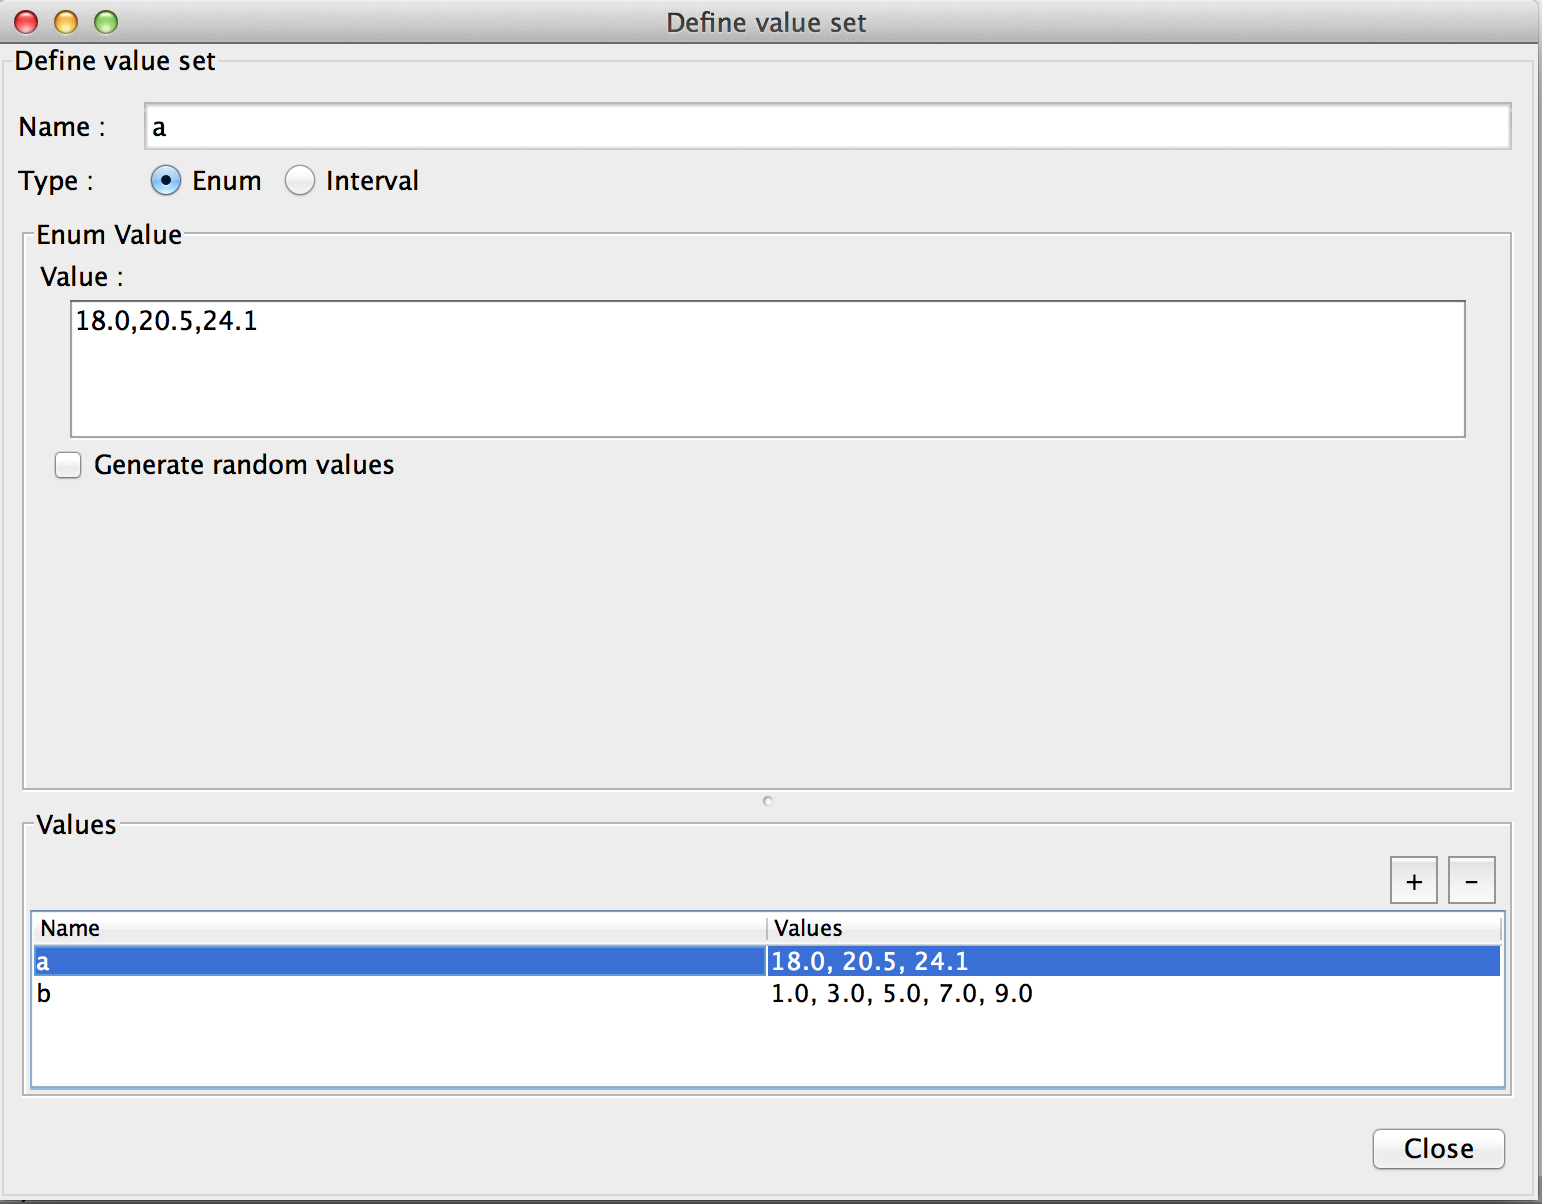
\includegraphics[width=\textwidth]{lr-value-set-a}
    \caption{{\tt a} of type enum}\label{fig:lr-value-set-a}
  \end{subfigure}
  \begin{subfigure}[b]{0.45\textwidth}
    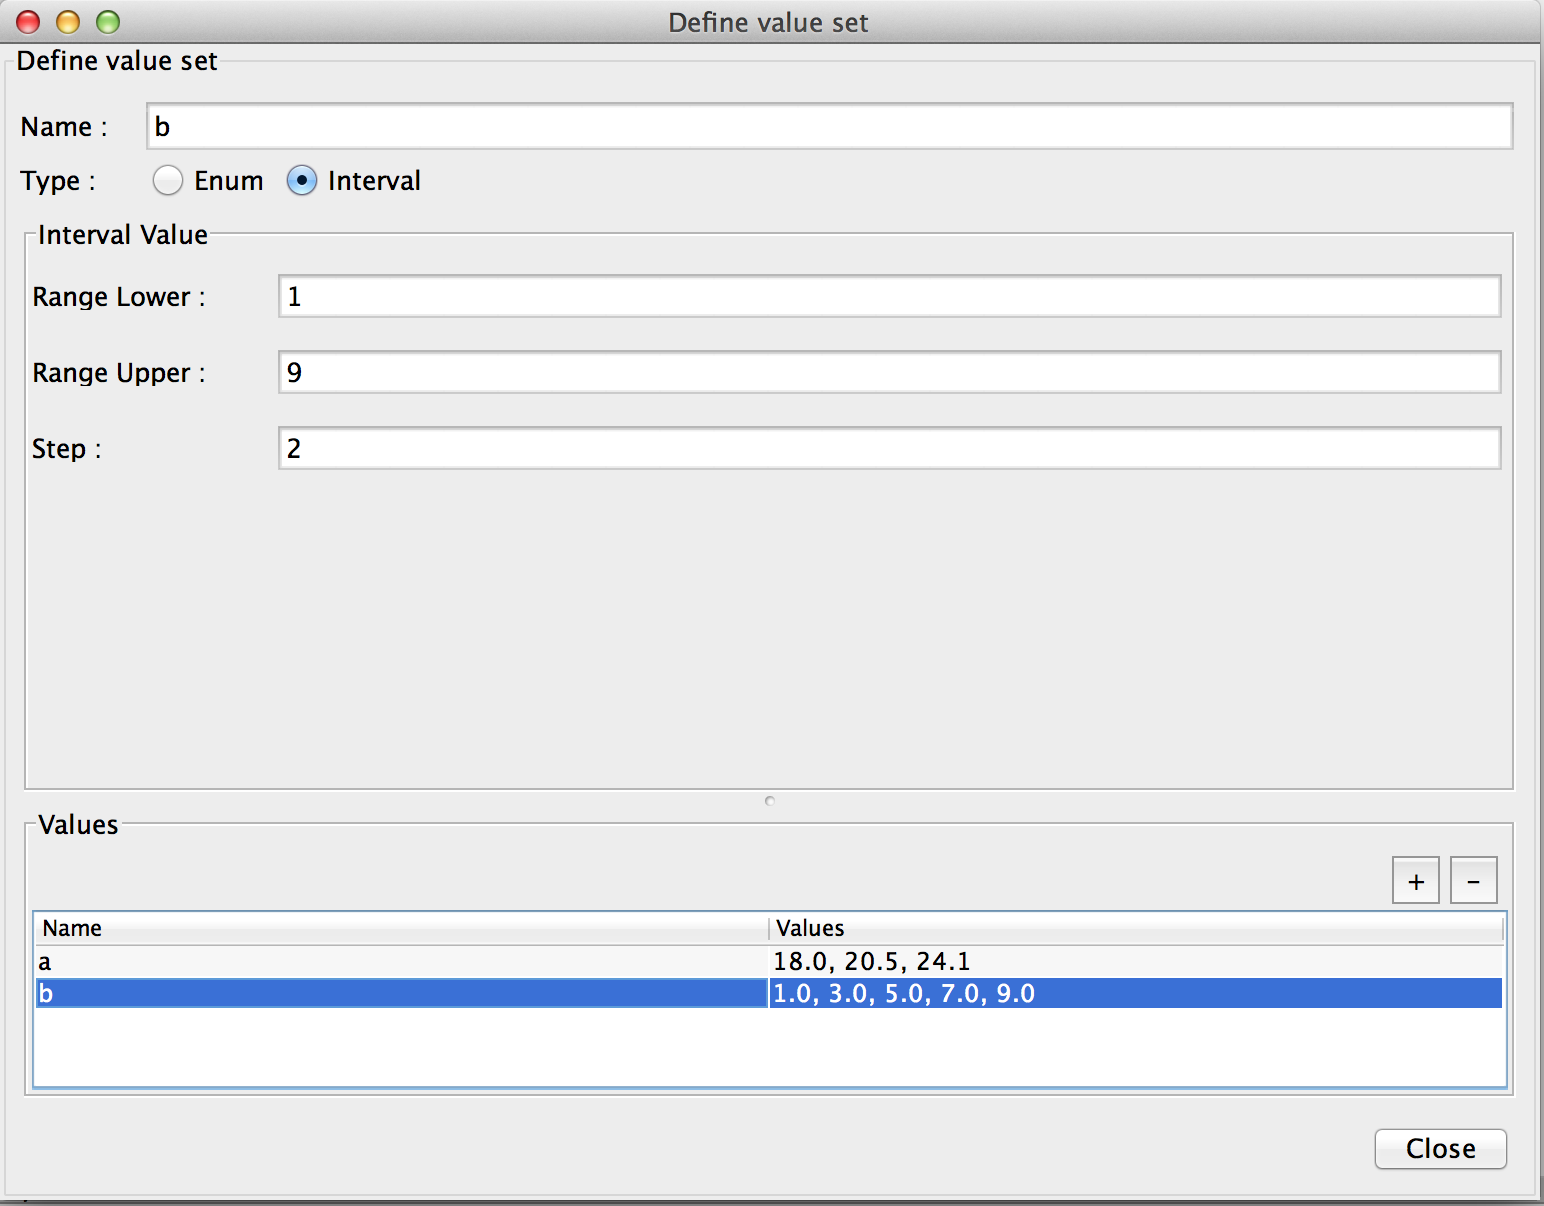
\includegraphics[width=\textwidth]{lr-value-set-b}
    \caption{{\tt b} of type interval}\label{fig:lr-value-set-b}
  \end{subfigure}
  \caption{Editing value-sets in the ``Define value set'' window.}\label{fig:lr-value-set}
\end{figure}

\subsubsection{Define a value-set}
In order to define or modify value-sets, push button ``Define value set'' at
first. Then a window will pop up. It allows users to define new value-set,
see existing value-sets, and modify them.

There are two types of value-sets: enum and interval. For a value-set of type
enum, each of possible values must be specified. On the other hand, only the
lower and upper (both inclusive) of a range of values with a step are required
to define a value-set of type interval.
Note that possible values of an enum should be separated by a comma.

\subsubsection{Use value-sets}
Once users have defined a value-set, it is available in the ``Expression''
field of any row in the ``Parameters'' table. For example, users can specify
{\tt a+2*b} in the field if there exists a couple of value-set named {\tt a} and
{\tt b}.

\section{Starting simulation}
To start simulation, use the menu ``Control''$\rightarrow$``Run'' or button
``Run'' on the control panel. It kicks simulation jobs for all loaded models.
Users can monitor the progress in total on the control panel, as well as the
one for a single job on the detail windows like Fig.~\ref{fig:lr-detail}.
\FigureOfImage{lr-detail}{The detail window during simulation.}

\section{Controlling simulation jobs}
After starting simulation jobs, users can control them instead of just waiting
for them finishing.

\subsection{Cancel jobs}
There are two ways to cancel running jobs; one is pushing the cross mark on
the control panel (see Fig.~\ref{fig:lr-progress}), which cancels all of related
jobs. The other is pushing the cross mark at the detail window, which cancels the
corresponding job only.
\FigureOfImage{lr-progress}{The progress bar / cross mark / ``Detail'' button on
 the control panel.}

\subsection{Pause and resume jobs}
As in Fig.~\ref{fig:control}, users can pause jobs at any time during simulation
by using the menu ``Control''$\rightarrow$``Pause''. Resumeing paused jobs can
be done with the menu ``Control''$\rightarrow$``Resume''.
Note that these operation affects all of alive jobs simultaneously.
\FigureOfImage{control}{The Control Menu.}

\section{Visualizing simulation results}
Flint has a feature to show a line graph for the result of a simulation on the
fly, not only after its job finished, but also int the middle of ongoing
simulation.

From the detail window, users can display the plot window by clicking button
``View'' for each simulation job.

\subsection{Choose abscissa and ordinates}
In order to draw a line graph, users have to specify the abscissa and ordinates
by drag-and-dropping variables from the left side frame.
\FigureOfImage{lr-plot}{Selecting {\tt V} as a Y1 ordinate.}

If there are so many variables that some of them scroll out on a frame, a scroll
bar appears on the left edge of the frame. Besides scrolling them by wheeling
with mouse, especially on the left side frame, the focus can jump to a variable
by typing an alphabet key (i.e., \texttt{[A-z]}) which specifies the first
character of the variable's name.

\subsection{Configuration for gnuplot}
Pushing the ``Plot'' button calls gnuplot to draw a line graph with the
specified abscissa and ordinates. Users have to install gnuplot in advance, and
to specify the location of the gnuplot executable (see
section~\ref{sec:preference}).

\subsubsection{Options for gnuplot}
Users can control the following options for gnuplot in Tab ``Range'' or ``Legend'':
\begin{itemize}
\item Minimum and/or maximum value(s) for the abscissa ($X$) and/or ordinates ($Y1$/$Y2$)
\item Labels for the abscissa ($X$) and/or ordinates ($Y1$/$Y2$)
\item With or without the title
\end{itemize}
These will be enabled on next time plotting.
\FigureOfImage{lr-plot-target}{The ``Target'' tab.}
\FigureOfImage{lr-plot-range}{The ``Range'' tab.}
\FigureOfImage{lr-plot-legend}{The ``Legend'' tab.}
\FigureOfImage{lr-gnuplot}{The line graph generated by gnuplot.}

\subsubsection{Writing the line graph to a file}
It is possible to make gnuplot write the line graph to some file, as follows:
\begin{itemize}
\item choose Tab ``Target''.
\item check the ``file'' button.
\item select a file format and path to be written.
\item push button ``Plot''.
\end{itemize}
Then a dialog will inform users of the resulting status.

\subsubsection{Trouble shooting}
\begin{itemize}
\item Pushing button ``Plot'' with no response, check the gnuplot initialization
  file to load. It is called $\tt{.gnuplot}$ on Unix and macOS, and
  $\tt{GNUPLOT.INI}$ on other systems.
\end{itemize}

\section{Saving output data}
Users may save the resulting simulation data for later investigation.
\FigureOfImage{lr-detail-buttons}{Buttons to export data in the detail window.}

\subsection{Exporing data as CSV}
Flint can export the result data into a CSV file.
The header column contains the variable names as well as their unit name if any.

The procedure is as follows:
\begin{enumerate}
\item Open the ``Detail'' window
\item Push button ``Export'' (see Fig.~\ref{fig:lr-detail-buttons})
\item Choose a target filename \emph{ending with .csv or .txt} in the file dialog.
\end{enumerate}

\subsection{Exporting data as ISD}
Flint can also export the result data into a ISD file.
The ISD file format is a binary file format for preserving multi-variate data.

The procedure is as follows:
\begin{enumerate}
\item Open the ``Detail'' window
\item Push button ``Export'' (see Fig.~\ref{fig:lr-detail-buttons})
\item Choose a target filename \emph{which extension is neither .csv nor .txt}
  in the file dialog.
\end{enumerate}

\subsection{Exporting all data into a directory}
It is sometimes useful to export all data for simulation jobs into a directory.
The procedure is as follows:
\begin{enumerate}
\item Open the ``Detail'' window
\item Push button ``Export all'' (see Fig.~\ref{fig:lr-detail})
\item Choose a target directory in the file dialog.
\end{enumerate}

\subsection{Sending data to a Garuda gadget}
If Flint is enabled for the Garuda protocol (see subsection~\ref{subsec:Garuda}
about how to turn it on), and an Garuda gadget is able to receive data in CSV or
ISD, it is easy to send the result from Flint through the Garuda protocol as
follows:
\begin{enumerate}
\item Open the ``Detail'' window
\item Push button ``Send via Garuda'' (see Fig.~\ref{fig:lr-detail})
\item Choose a target gadget from the list in the next dialog.
\end{enumerate}

\section{Flint K3}
Instead of runnsing simulation with Flint, it is also possible to submit a loaded
model to Flint K3 (\url{https://flintk3.unit.oist.jp/}) for simulation.
A K3 account is necessary to use this advanced feature.

\subsection{From menu}
To submit a model to Flint K3,
\begin{enumerate}
\item Load a model
\item Select the menu ``Control''$\rightarrow$``Send to Flint K3''
\item Enter the User ID and Password of a K3 account and the title of new job
  (see Fig.~\ref{fig:new-job-to-k3})
\item Push button ``Submit''
\end{enumerate}
\FigureOfImage{new-job-to-k3}{The ``New job to K3'' dialog.}
Then a dialog will appear to tell whether it is done successfully or not.

\section{Exporting C source code from model}
Not only running online simulation, but also Flint can export simulation code
as a C99 source file from a loaded model. So far it works only for pure ODE models.

\subsection{From menu}
To export C code from a model,
\begin{enumerate}
\item Load a model
\item Select the menu ``File''$\rightarrow$``Export''$\rightarrow$``C''
\item Choose a target filename via the file dialog that follows.
\end{enumerate}
\FigureOfImage{export-to-c}{The menu ``File''$\rightarrow$``Export''$\rightarrow$``C''.}
Then a dialog will appear to tell whether it is done successfully or not.

Please note that the numerical method used in the exported code is the one
specified in the original model, e.g., Euler or Runge-Kutta 4th-order method;
the ARKode solver of SUNDIALS has not been supported yet.

\subsection{How to build a program from exported code}
Once a C source file exported, what to do next is building the program by a C compiler
conforming C99 standard.

If, for example, gcc is available, then invoking the following code
\begin{verbatim}
$ gcc -O3 -std=c99 -o simulate exported.c
\end{verbatim}
will produce an executable named {\tt simulate} from the C source file {\tt exported.c}.

Finally,
\begin{verbatim}
$ ./simulate output.isd
\end{verbatim}
will run a simulation, writing the whole output into {\tt output.isd}.

\section{Preference}
\label{sec:preference}
Users can customize Flint's preference.

\subsection{Plotter}
This is an advanced option.
For gnuplot, select the path of {\tt gnuplot} (or {\tt pgnuplot.exe} on Windows),
e.g., ``$\tt{/usr/bin/gnuplot}$''. On macOS, say,
{\tt /Applications/gnuplot.app} as an application bundle of gnuplot, its value
should be \[{\tt /Applications/gnuplot.app/bin/gnuplot}.\]
\FigureOfImage{preference-plotter}{The ``Plotter'' panel on the preference dialog.}

\subsection{Garuda}
\label{subsec:Garuda}
Turning it on makes Flint enabled for the Garuda protocol on the desktop, like
Fig.~\ref{fig:preference-garuda}.
\FigureOfImage{preference-garuda}{The ``Garuda'' panel on the preference dialog.}

\section{Shortcut keys}
There are useful shortcut keys as follows:

\subsection{Keys for main menu}
\begin{tabular}{l||c|c}
  Command & Shortcut keys on macOS & Shortcut keys on Linux or Windows\\
  \hline
  File $\rightarrow$ Open & {\tt Cmd}+O & {\tt Ctrl}+O \\
  File $\rightarrow$ Exit & {\tt Cmd}+Q & {\tt Ctrl}+Q \\
  Edit $\rightarrow$ Copy & {\tt Cmd}+C & {\tt Ctrl}+C \\
  File $\rightarrow$ Cut  & {\tt Cmd}+X & {\tt Ctrl}+X \\
  Edit $\rightarrow$ Preference & {\tt Cmd}+, & {\tt Ctrl}+, \\
  Control $\rightarrow$ Run & {\tt Option}+R & {\tt Alt}+R \\
  Control $\rightarrow$ Pause & {\tt Option}+P & {\tt Alt}+P \\
  Control $\rightarrow$ Resume & {\tt Option}+S & {\tt Alt}+S \\
\end{tabular}

\subsection{Additional keys}
Both {\tt Esc} and {\tt Ctrl}+{\tt W} (or {\tt Cmd}+{\tt W} on Mac) can close an active
subwindow in which there is no dedicated button to close it.

%%%%%%%%%%%%%%%%%%%%%%%%%%%%%%%%%%%%%%%%%%%%%%%%%%%%%%%%%%%%%%%%%%%%%%%%

\chapter{Command Line Interface}
\Flint\ allows users to run a simulation in a command shell.

\section{Launching Flint}

\subsection{Invocation with no arguments}
It is possible to launch Flint with the command {\tt open(1)} of macOS as follows:
\begin{verbatim}
$ open Flint.app
\end{verbatim}
Note that it does nothing but launches the graphical user interface of Flint.
In a {\tt cmd} session on Windows,
\begin{verbatim}
$ flint.exe
\end{verbatim}
has the similar effect.

\subsection{Invocation with filenames}
If filenames of models are given in the command line on Windows:
\begin{verbatim}
$ flint.exe model1 model2 ...
\end{verbatim}
then Flint tries to open them immediately after launching the GUI.

\section{Showing help}
Specifying {\tt -help} in the command line shows the help message.

\subsection{Synopsis}
On Windows:
\begin{verbatim}
$ flint.exe -help
\end{verbatim}

\section{Running a simulation: the headless mode}
Specifying {\tt -headless} in the command line enable the headless mode, which
runs a simulation of given model with the default configuration.

\subsection{Synopsis}
On Windows:
\begin{verbatim}
$ flint.exe -headless input output [-e file] [-g n] [-s file]
\end{verbatim}
Load a model at {\tt input}, simulation it with the default configuration,
and leave the result at {\tt output}.
The following suboptions are available:
\begin{description}
\item[-e {\tt file}] \hfill \\
  save error messages during simulation as {\tt file}.
\item[-g {\tt n}] \hfill \\
  specify a sampleing rate i.e. 1 output per {\tt n} step.
\item[-s {\tt file}] \hfill \\
  specify output variables with {\tt file}.
\end{description}


%%%%%%%%%%%%%%%%%%%%%%%%%%%%%%%%%%%%%%%%%%%%%%%%%%%%%%%%%%%%%%%%%%%%%%%%

\chapter{Frequently Asked Questions (FAQ)}
Please read this chapter first when in doubt.

\section{On Windows}
\subsubsection{Failure at loading a model}
If the error message shows an error message like
\begin{verbatim}
'flint-open' is not recognized as an internal or external command,
operable program or batch file.
\end{verbatim}
then make sure that the PATH environment variable contains
\begin{verbatim}
C:\Program Files (x86)\Flint\
\end{verbatim}
and try Flint again after rebooting Windows.

\end{document}
